\documentclass{standalone}
\usepackage{tikz}
\usetikzlibrary{patterns, positioning}
\usepackage[sfdefault]{ClearSans} %% option 'sfdefault' activates Clear Sans as the default text font
\usepackage[T1]{fontenc}

\begin{document}
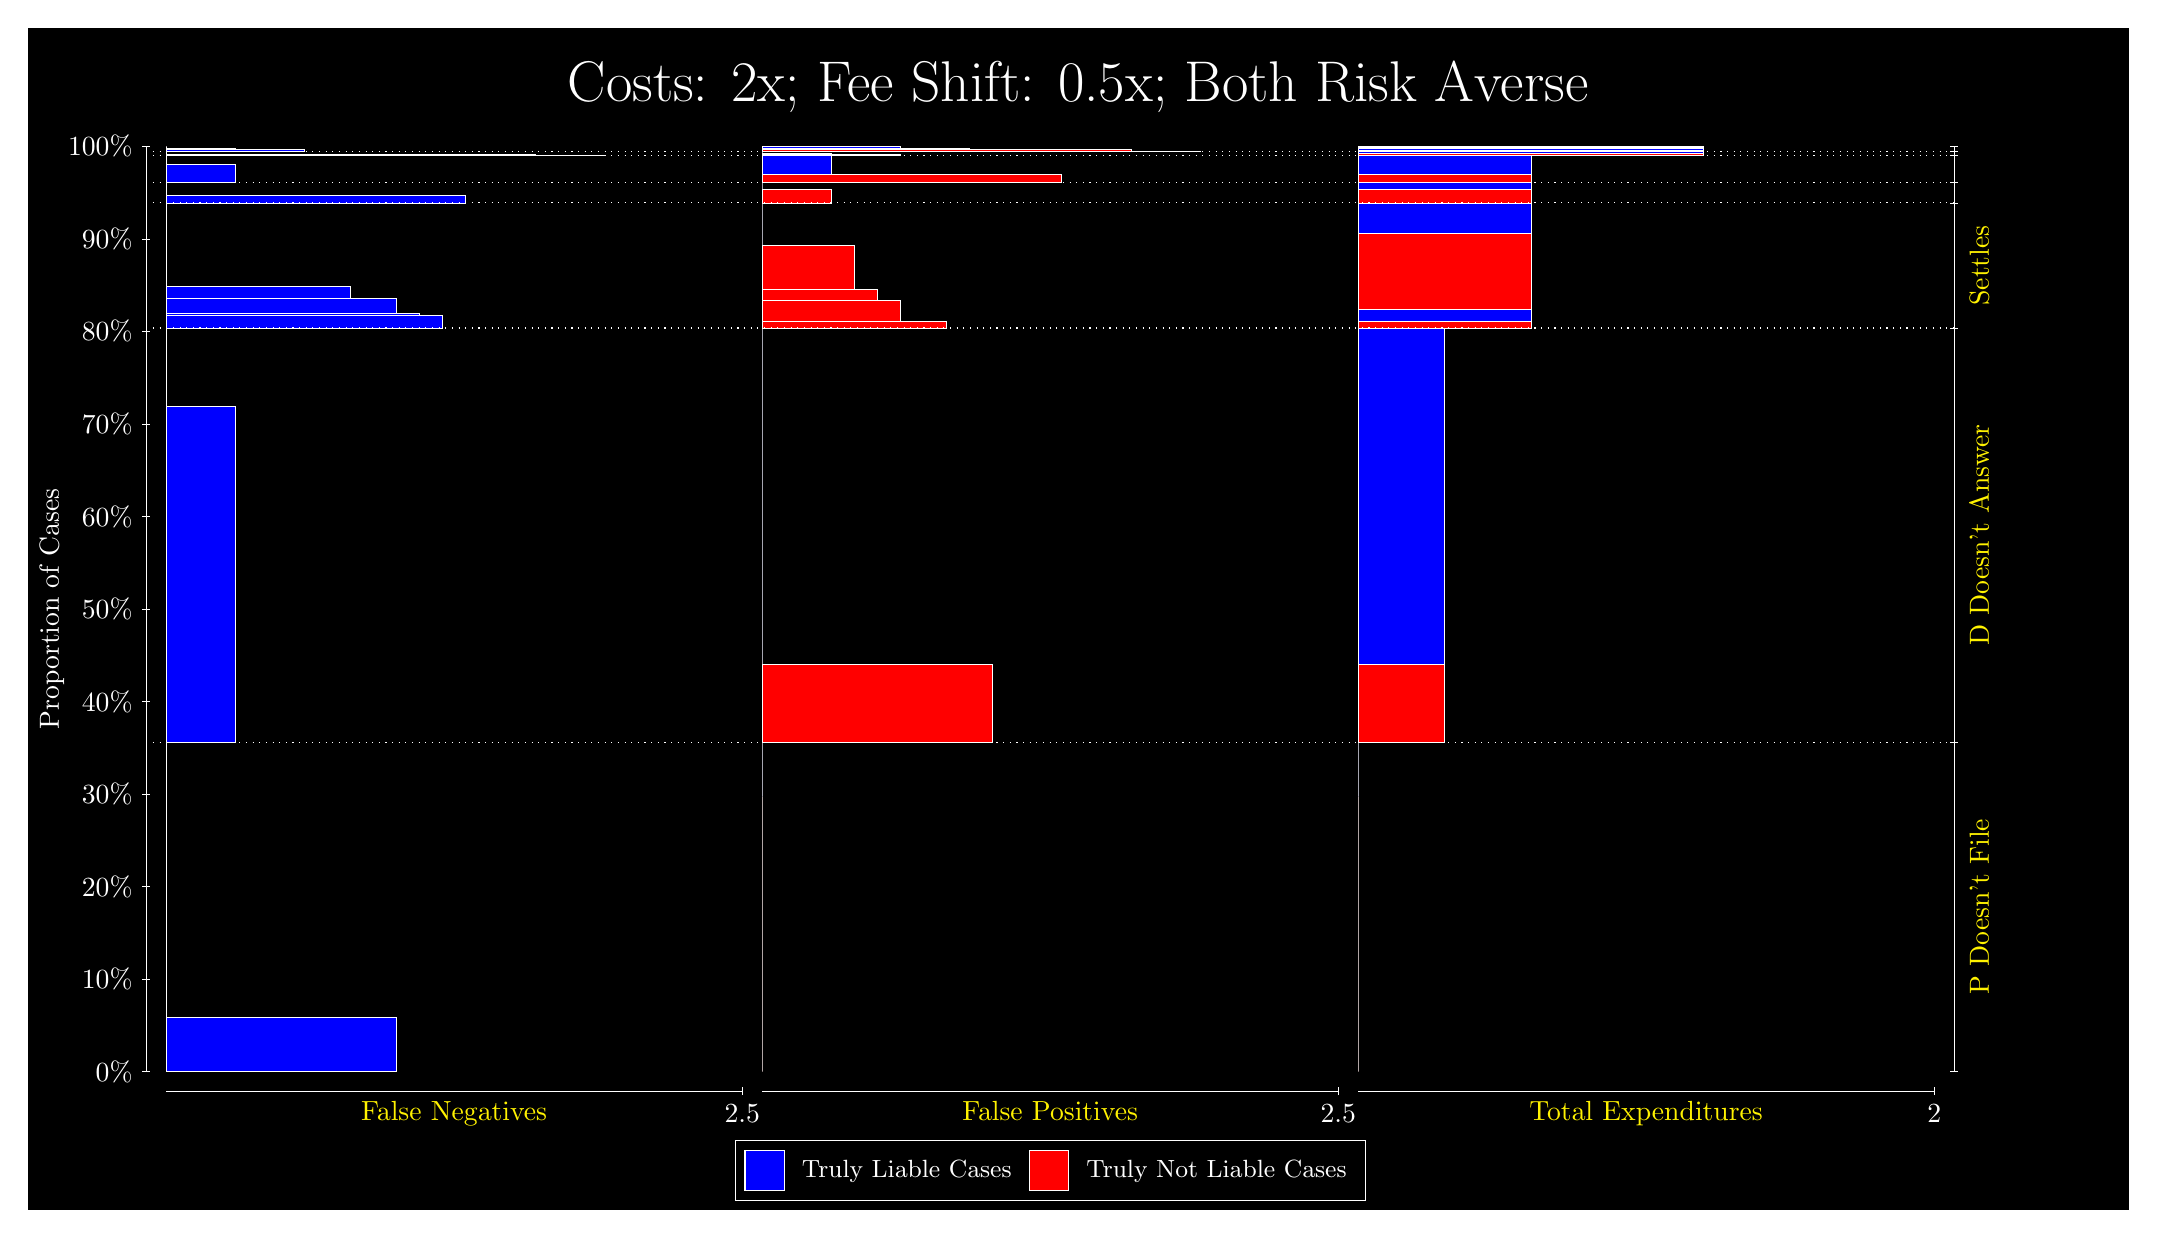
\begin{tikzpicture}
\draw[fill=black] (0,0) rectangle (26.667,15);
\draw[text=white] (0,13.5) rectangle (26.667,15) node[midway] {\huge Costs: 2x; Fee Shift: 0.5x; Both Risk Averse};
\draw[white, very thin] (1.5,1.75) -- (1.5,13.5);
\node[rotate=90, text=white, anchor=center] at (0.3, 7.625) {Proportion of Cases};
\draw[white, very thin] (1.45,1.75) -- (1.55,1.75);
\node[text=white, anchor=east] at (1.45, 1.75) {0\%};
\draw[white, very thin] (1.45,2.925) -- (1.55,2.925);
\node[text=white, anchor=east] at (1.45, 2.925) {10\%};
\draw[white, very thin] (1.45,4.1) -- (1.55,4.1);
\node[text=white, anchor=east] at (1.45, 4.1) {20\%};
\draw[white, very thin] (1.45,5.275) -- (1.55,5.275);
\node[text=white, anchor=east] at (1.45, 5.275) {30\%};
\draw[white, very thin] (1.45,6.45) -- (1.55,6.45);
\node[text=white, anchor=east] at (1.45, 6.45) {40\%};
\draw[white, very thin] (1.45,7.625) -- (1.55,7.625);
\node[text=white, anchor=east] at (1.45, 7.625) {50\%};
\draw[white, very thin] (1.45,8.8) -- (1.55,8.8);
\node[text=white, anchor=east] at (1.45, 8.8) {60\%};
\draw[white, very thin] (1.45,9.975) -- (1.55,9.975);
\node[text=white, anchor=east] at (1.45, 9.975) {70\%};
\draw[white, very thin] (1.45,11.15) -- (1.55,11.15);
\node[text=white, anchor=east] at (1.45, 11.15) {80\%};
\draw[white, very thin] (1.45,12.325) -- (1.55,12.325);
\node[text=white, anchor=east] at (1.45, 12.325) {90\%};
\draw[white, very thin] (1.45,13.5) -- (1.55,13.5);
\node[text=white, anchor=east] at (1.45, 13.5) {100\%};

\draw[white, very thin] (24.457,1.75) -- (24.457,13.5);
\draw[white, very thin] (24.407,1.75) -- (24.507,1.75);
\node[anchor=west] at (24.407, 1.75) {};
\draw[white, very thin] (24.407,5.9328) -- (24.507,5.9328);
\node[anchor=west] at (24.407, 5.9328) {};
\draw[white, very thin] (24.407,11.193) -- (24.507,11.193);
\node[anchor=west] at (24.407, 11.193) {};
\draw[white, very thin] (24.407,12.782) -- (24.507,12.782);
\node[anchor=west] at (24.407, 12.782) {};
\draw[white, very thin] (24.407,13.044) -- (24.507,13.044);
\node[anchor=west] at (24.407, 13.044) {};
\draw[white, very thin] (24.407,13.38) -- (24.507,13.38);
\node[anchor=west] at (24.407, 13.38) {};
\draw[white, very thin] (24.407,13.439) -- (24.507,13.439);
\node[anchor=west] at (24.407, 13.439) {};
\draw[white, very thin] (24.407,13.5) -- (24.507,13.5);
\node[anchor=west] at (24.407, 13.5) {};

\draw[white, very thin, fill=blue] (1.75,1.75) rectangle (4.6775,2.4407);
\draw[white, very thin, fill=red] (1.75,2.4407) rectangle (1.75,5.9328);
\draw[white, very thin, fill=blue] (1.75,5.9328) rectangle (2.6283,10.198);
\draw[white, very thin, fill=red] (1.75,10.198) rectangle (1.75,11.193);
\draw[white, very thin, fill=blue] (1.75,11.193) rectangle (5.2631,11.355);
\draw[white, very thin, fill=blue] (1.75,11.355) rectangle (4.9703,11.383);
\draw[white, very thin, fill=blue] (1.75,11.383) rectangle (4.6775,11.572);
\draw[white, very thin, fill=blue] (1.75,11.572) rectangle (4.092,11.725);
\draw[white, very thin, fill=red] (1.75,11.725) rectangle (1.75,12.782);
\draw[white, very thin, fill=blue] (1.75,12.782) rectangle (5.5558,12.874);
\draw[white, very thin, fill=red] (1.75,12.874) rectangle (1.75,13.044);
\draw[white, very thin, fill=blue] (1.75,13.044) rectangle (2.6283,13.278);
\draw[white, very thin, fill=red] (1.75,13.278) rectangle (1.75,13.38);
\draw[white, very thin, fill=blue] (1.75,13.38) rectangle (7.3123,13.384);
\draw[white, very thin, fill=blue] (1.75,13.384) rectangle (6.4341,13.4);
\draw[white, very thin, fill=red] (1.75,13.4) rectangle (1.75,13.439);
\draw[white, very thin, fill=blue] (1.75,13.439) rectangle (3.5065,13.463);
\draw[white, very thin, fill=blue] (1.75,13.463) rectangle (2.6283,13.479);
\draw[white, very thin, fill=red] (1.75,13.479) rectangle (1.75,13.5);
\draw[white, very thin, fill=red] (9.3189,1.75) rectangle (9.3189,5.2421);
\draw[white, very thin, fill=blue] (9.3189,5.2421) rectangle (9.3189,5.9328);
\draw[white, very thin, fill=red] (9.3189,5.9328) rectangle (12.246,6.9278);
\draw[white, very thin, fill=blue] (9.3189,6.9278) rectangle (9.3189,11.193);
\draw[white, very thin, fill=red] (9.3189,11.193) rectangle (11.661,11.281);
\draw[white, very thin, fill=red] (9.3189,11.281) rectangle (11.075,11.546);
\draw[white, very thin, fill=red] (9.3189,11.546) rectangle (10.783,11.683);
\draw[white, very thin, fill=red] (9.3189,11.683) rectangle (10.49,12.249);
\draw[white, very thin, fill=blue] (9.3189,12.249) rectangle (9.3189,12.782);
\draw[white, very thin, fill=red] (9.3189,12.782) rectangle (10.197,12.952);
\draw[white, very thin, fill=blue] (9.3189,12.952) rectangle (9.3189,13.044);
\draw[white, very thin, fill=red] (9.3189,13.044) rectangle (13.125,13.146);
\draw[white, very thin, fill=blue] (9.3189,13.146) rectangle (10.197,13.38);
\draw[white, very thin, fill=red] (9.3189,13.38) rectangle (11.075,13.403);
\draw[white, very thin, fill=red] (9.3189,13.403) rectangle (10.197,13.418);
\draw[white, very thin, fill=blue] (9.3189,13.418) rectangle (9.3189,13.439);
\draw[white, very thin, fill=red] (9.3189,13.439) rectangle (14.881,13.443);
\draw[white, very thin, fill=red] (9.3189,13.443) rectangle (14.003,13.459);
\draw[white, very thin, fill=blue] (9.3189,13.459) rectangle (11.954,13.476);
\draw[white, very thin, fill=blue] (9.3189,13.476) rectangle (11.075,13.5);
\draw[white, very thin, fill=red] (16.888,1.75) rectangle (16.888,5.2421);
\draw[white, very thin, fill=blue] (16.888,5.2421) rectangle (16.888,5.9328);
\draw[white, very thin, fill=red] (16.888,5.9328) rectangle (17.986,6.9278);
\draw[white, very thin, fill=blue] (16.888,6.9278) rectangle (17.986,11.193);
\draw[white, very thin, fill=red] (16.888,11.193) rectangle (19.083,11.281);
\draw[white, very thin, fill=blue] (16.888,11.281) rectangle (19.083,11.434);
\draw[white, very thin, fill=red] (16.888,11.434) rectangle (19.083,12.402);
\draw[white, very thin, fill=blue] (16.888,12.402) rectangle (19.083,12.782);
\draw[white, very thin, fill=red] (16.888,12.782) rectangle (19.083,12.952);
\draw[white, very thin, fill=blue] (16.888,12.952) rectangle (19.083,13.044);
\draw[white, very thin, fill=red] (16.888,13.044) rectangle (19.083,13.146);
\draw[white, very thin, fill=blue] (16.888,13.146) rectangle (19.083,13.38);
\draw[white, very thin, fill=red] (16.888,13.38) rectangle (21.279,13.418);
\draw[white, very thin, fill=blue] (16.888,13.418) rectangle (21.279,13.439);
\draw[white, very thin, fill=red] (16.888,13.439) rectangle (21.279,13.454);
\draw[white, very thin, fill=blue] (16.888,13.454) rectangle (21.279,13.479);
\draw[white, very thin, fill=red] (16.888,13.479) rectangle (21.279,13.483);
\draw[white, very thin, fill=blue] (16.888,13.483) rectangle (21.279,13.5);
\draw[white, dotted] (1.5,5.9328) -- (24.457,5.9328);
\draw[white, dotted] (1.5,11.193) -- (24.457,11.193);
\draw[white, dotted] (1.5,12.782) -- (24.457,12.782);
\draw[white, dotted] (1.5,13.044) -- (24.457,13.044);
\draw[white, dotted] (1.5,13.38) -- (24.457,13.38);
\draw[white, dotted] (1.5,13.439) -- (24.457,13.439);
\draw[white, very thin] (1.75,1.5) -- (9.0689,1.5);
\node[text=yellow, anchor=north] at (5.4094, 1.5) {False Negatives};
\draw[white, very thin] (9.0689,1.45) -- (9.0689,1.55);
\node[text=white, anchor=north] at (9.0689, 1.45) {2.5};

\draw[white, very thin] (9.3189,1.5) -- (16.638,1.5);
\node[text=yellow, anchor=north] at (12.978, 1.5) {False Positives};
\draw[white, very thin] (16.638,1.45) -- (16.638,1.55);
\node[text=white, anchor=north] at (16.638, 1.45) {2.5};

\draw[white, very thin] (16.888,1.5) -- (24.207,1.5);
\node[text=yellow, anchor=north] at (20.547, 1.5) {Total Expenditures};
\draw[white, very thin] (24.207,1.45) -- (24.207,1.55);
\node[text=white, anchor=north] at (24.207, 1.45) {2};

\node[text=yellow, centered, rotate=90] at (24.777, 3.8414) {P Doesn't File};
\node[text=yellow, centered, rotate=90] at (24.777, 8.5627) {D Doesn't Answer};
\node[text=yellow, centered, rotate=90] at (24.777, 11.987) {Settles};





\draw (12.978300999999998,1.5) node[draw=none] (baseCoordinate) {};
\begin{scope}[align=center]
        \matrix[scale=0.5, draw=white, below=0.5cm of baseCoordinate, nodes={draw}, column sep=0.1cm]{
            \node[rectangle, draw, minimum width=0.5cm, minimum height=0.5cm, fill=blue] {}; &
            \node[draw=none, font=\small, text=white] (B) {Truly Liable Cases}; &
            \node[rectangle, draw, minimum width=0.5cm, minimum height=0.5cm, fill=red] {}; &
            \node[draw=none, font=\small, text=white] (B) {Truly Not Liable Cases}; \\
            };
\end{scope}

\end{tikzpicture}
\end{document}